\documentclass[legalpaper,12pt,addpoints]{exam}
\usepackage[utf8]{inputenc}
\usepackage[english]{babel}
\usepackage{graphicx}
\usepackage[none]{hyphenat}
\usepackage[top=1in, bottom=1in, left=0.75in, right=0.75in]{geometry}
\usepackage{amsmath,amssymb}
\usepackage{wrapfig}
\usepackage{comment}
\usepackage{multicol}
\usepackage{multirow}
\usepackage{graphicx}
\usepackage{upgreek} % para poner letras griegas sin cursiva
\usepackage{cancel} % para tachar
\usepackage{mathdots} % para el comando \iddots
\usepackage{mathrsfs} % para formato de letra
\usepackage{stackrel} % para el comando \stackbin
\usepackage{pstricks}
\usepackage{marginnote}
\usepackage{tcolorbox}
\tcbuselibrary{theorems}
\usepackage{circuitikz}
\usepackage{tikz}
\usepackage{pdfpages}

\newcommand{\university}{Universidad del B\'io-B\'io }
\newcommand{\faculty}{Facultad de Ciencias}
\newcommand{\class}{F\'isica II - Electromagnetismo}
%\newcommand{\class}{F\'isica I M\'odulo 2}
\newcommand{\examnum}{\textbf{Certamen 2 }}
\newcommand{\content}{Campos Magnéticos por Biot-Savart y Ampere y Ley de Inducción de Faraday Lenz}
%\newcommand{\examdate}{\today}
\newcommand{\examdate}{Abril 9, 2025}
\newcommand{\timelimit}{80 minutos}

\pagestyle{headandfoot}
\firstpageheader{}{}{}
\firstpagefooter{}{Page \thepage\ of \numpages}{}
\runningheader{\class}{\examnum}{\examdate}
\runningheadrule
\runningfooter{}{Page \thepage\ of \numpages}{}
\begin{document}
%%%%% PORTADA %%%%
\begin{comment}
    

	\pointname{}
	\boxedpoints
	
	\title{
		\begin{center}
			
\includegraphics[width=8cm]{figs/cienciasubb.png}\\
			%\Large{\textbf{Certamen 2}}\\
			%Ondas Electromagn'eticas  Ing.Civil El'ectrica UCSC 2021-02\\
		\end{center}
		\class \\  \examnum}
	\date{Octubre 20, 2025}
	\maketitle
	\begin{flushleft}
		\makebox[17cm]{\textbf{Nombre}:\ \hrulefill }\\
		\vspace{1cm}
		\makebox[17cm]{\textbf{Rut}:\ \hrulefill \textbf{Folio}:\ \hrulefill}
	\end{flushleft}
	\noindent \rule{\textwidth}{1pt}
 
\vspace{0.3cm}	
\begin{minipage}[c]{16cm}
    \noindent \textbf{Algunas consideraciones para esta evaluación:}
 \begin{itemize}
 \begin{small}
     \item El certamen 1 contiene \numpages\ páginas (incluida la portada) y \numquestions\ preguntas, con un total de \numpoints puntos.
     \item Cada pregunta debe ser respondida por sólo una respuesta. En caso de presentar más de una, se anulan las respuestas.
     \item No está permitido el uso de celulares o tablet en el desarrollo de esta evaluación. De ser sorprendido utilizando estos artículos su evaluación será califica con nota 1.0.
     \item Buena suerte!
      \end{small}
 \end{itemize}
\end{minipage}
 
 

%%%%%%%%%%%%%% nombre de los profes

\begin{table}[h]
\begin{center}
\begin{tabular}{ccccc}
\multicolumn{5}{l}{\noindent Seleccione con una \textbf{X} el nombre del profesor de su sección:}\\ \cline{1-2} \cline{4-5} 
\multicolumn{1}{|p{5.5cm}|}{Prof. Luis Soto}                      & \multicolumn{1}{p{1.5cm}|}{} & \multicolumn{1}{p{1.0cm}|}{} & \multicolumn{1}{p{5.5cm}|}{Prof. Natalia Molina}     & \multicolumn{1}{p{1.5cm}|}{} \\ \cline{1-2} \cline{4-5} 
\multicolumn{1}{|p{5.5cm}|}{Prof. Evelyn Riveros}                  & \multicolumn{1}{p{1.5cm}|}{} & \multicolumn{1}{p{1.5cm}|}{} & \multicolumn{1}{p{5.5cm}|}{Prof. Ricardo Espinoza}       & \multicolumn{1}{p{1.5cm}|}{} \\ \cline{1-2} \cline{4-5} 
\multicolumn{1}{|p{5.5cm}|}{Prof. Bayron Cerda}                  & \multicolumn{1}{p{1.5cm}|}{} & \multicolumn{1}{p{1.5cm}|}{} & \multicolumn{1}{p{5.5cm}|}{Prof. Cristobal Gatica}       & \multicolumn{1}{p{1.5cm}|}{} \\ \cline{1-2} \cline{4-5} 
%\\ \cline{1-2} \cline{4-5} 
\multicolumn{1}{|p{5.5cm}|}{Prof. Luis Liempi}                  & \multicolumn{1}{p{1.5cm}|}{} & \multicolumn{1}{p{1.5cm}|}{} & \multicolumn{1}{p{5.5cm}|}{}       & \multicolumn{1}{p{1.5cm}|}{} \\ \cline{1-2} \cline{4-5} 
\end{tabular}
\end{center}
\end{table}





	\begin{center}
		\large{
			\textbf{Puntaje}\\
			\medskip
			%\combinedgradetable[v][questions]}
                 \gradetable[v][questions]}
	\end{center}
	
	
	\clearpage
%%%% fin portada
\end{comment}    
    
	\begin{questions}

%----------- PROBLEMA 2 --------
 %--------------- Fuerza magnetica y ley de Ampere ------------
		%\begin{comment}
\begin{minipage}[c]{10cm}
  \question[19] Se dispone de un sistema formado por 3 cargas puntuales: $q_1=-12[nC]$, $q_2=25[nC]$ y $q_3=-6[nC]$ ubicadas en los puntos $P_1(0,6,6)$, $P_2(4,0,3)$ y $P_3(4,4,4)$ respectivamente. Considere que las posiciones de las cargas están medidas en centímetros y el valor de  $K=9\times10^9[Nm^2/C^2]$, responda\\
  Nota:\\
  prefijos: $c=10^{-2}$, $m=10^{-3}$, $\mu=10^{-6}$, $n=10^{-9}$, $p=10^{-12}$.
   \end{minipage}
   \hspace{1cm}
   %Figura certamen
   \begin{minipage}[c]{6cm}
    \centering
    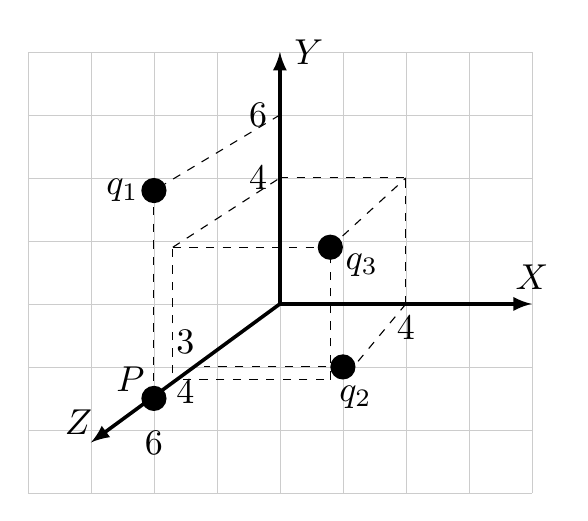
\begin{tikzpicture}[scale=0.8]
 \draw[step=1cm,very thin, gray!40] (-4,-3) grid (4,4);
    %  \draw[line width=1.4,dashed,gray] (0,0) circle (3);
      \draw[black, line width =1.3,->, >=latex] (0,0) -- (0,4) node [black, right, scale=1.3] {$Y$};
       \draw[black, line width =1.3,->, >=latex] (0,0) -- (4,0) node [black, above, scale=1.3] {$X$};
       \draw[black,line width=1.3, ->, >=latex] (0,0) -- (-3,-2.2) node [black, above,scale=1.3] at (-3.2,-2.3) {$Z$};
     
       %P
      \node[black, right, scale=1.3,right] at (-2.8,-1.2) {$P$};
     \fill (-2,-1.5) circle (0.2);
    %   \node[black, scale=1.3] at (-1.4,-1.5) {$3$};
       % \fill (0,-3) circle (0.2);
 \node[black, scale=1.3,left] at (0,3) {$6$};
 %q_1
     \fill (-2,1.8) circle (0.2);
    \draw[black, dashed] (0,3) -- (-2,1.8) node[black, scale=1.3] at (-2.5,1.8) {$q_1$};
\draw[black, dashed] (-2,1.8) -- (-2,-1.5) node[black, scale=1.3] at (-2,-2.2) {$6$};
    
 %  \draw[black, dashed] (0,3) -- (2,4) node[black, scale=1.3, xshift=-10pt] at (0,4) {$8$}; 
 
 %q_2
%\fill (0,4) circle (0.2);
  \draw[black, dashed] (2,0) -- (1,-1.2) node[black, below, scale=1.3] at (2,0) {$4$}; 
  \draw[black, dashed] (1,-1) -- (-1.2,-1) node[black, scale=1.3] at (-1.5,-0.6) {$3$};
  \fill (1,-1) circle (0.2);
\node[black, scale=1.3,below] at (1.2,-1.1) {$q_2$};

 %q_3 
\draw[black, dashed] (0,2) -- (2,2) node[black, left, scale=1.3] at (0,2) {$4$};
\draw[black, dashed] (2,0) -- (2,2); %node[black, right, scale=1] at (0,2) {$4$};
%\draw[black, dashed] (0.5,-1.2) -- (-1.5,-1.2);
\draw[black, dashed] (0.7,-1.2) -- (-1.6,-1.2) node[black, scale=1.3] at (-1.5,-1.4) {$4$};
\draw[black, dashed] (0.8,0.9) -- (2,2);
\draw[black, dashed] (0.8,-1.2) -- (0.8,0.9);
\draw[black, dashed] (-1.7,-1.1) -- (-1.7,0.9);
\draw[black, dashed] (-1.7,0.9) -- (0.8,0.9);
\draw[black, dashed] (-1.7,0.9) -- (0,2);
\node[black, scale=1.3,below] at (1.3,1) {$q_3$};
\fill (0.8,0.9) circle (0.2);
 % \fill (-1.3,1) circle (0.2);
 % \draw[black, dashed] (1.5,0) -- (1.5,-0.5) node[black, right, scale=1.3] at (-1.3,-0.3) {$2$};
   \end{tikzpicture}
\end{minipage}
    \begin{parts}
        \part {\bf\red{(8.0 pts)}} calcule el potencial eléctrico en un punto P(0,0,6)
        \vspace{8cm}
        \part {\bf\red{(8.0 pts)}} calcule la energía contenida en el sistema.
        \vspace{8cm}
        \part {\bf\red{(3.0 pts)}} calcule el trabajo necesario en traer una carga $q_4=14[nC]$ al punto P.
        \vspace{4cm}
        \end{parts}
 
%\end{comment}

% \begin{comment}
\newpage
%%%%%%%%%%%%%%%%%    PAUTA PROBLEMA 3 %%%%%%%%
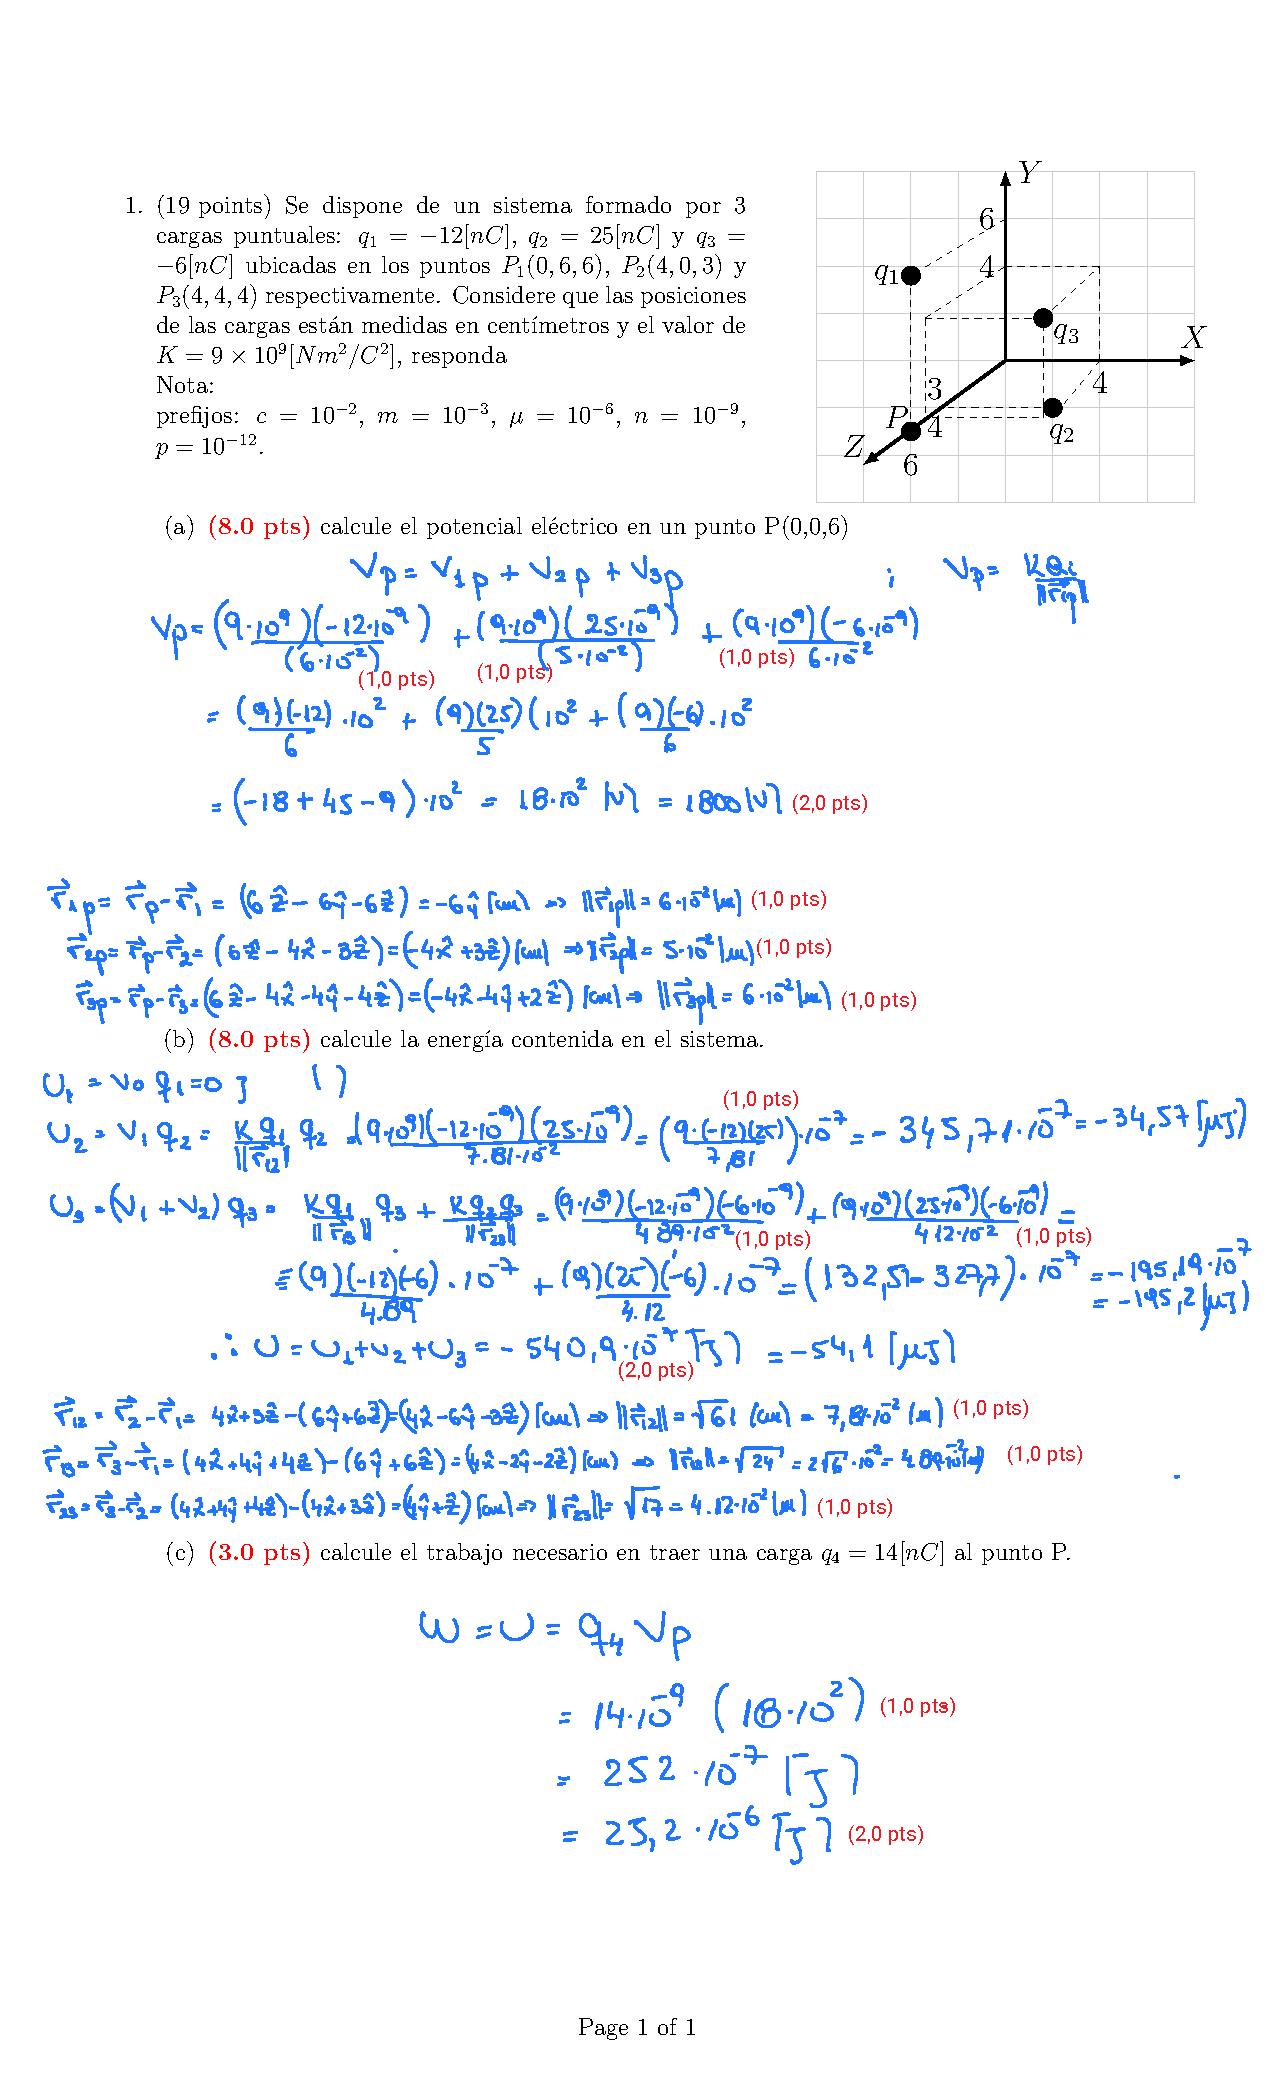
\includepdf[pages=1-1]{Pauta-P2_B__C2_ELECTRO_UBB_S2_2026.pdf}


%\end{comment}





		
	
	\end{questions}
\end{document}
